The first step when we are designing a system's architecture is to know its input and output. In this case, we want to implement a natural language processing system that analyses the writing style of e-mails. As we have previously mentioned, the stylometric analysis will be represented through chosen style markers. Therefore, our system's output is going to be that chosen metrics (they are explained in section \ref{section:measmod}) of each message.

In respect of the system's input, because of the nature of the problem we face, it is reasonable to think that it must be an e-mail. However, we do not have the corpus of e-mails to analyse. For this reason, our first step will be to extract the e-mails that will be analysed. Hence, our system's input is going to be the information of the Gmail user for accessing to the data that we are interested in. Therefore, we are going to develop a system which receives some information of a Gmail user as input and obtains different metrics for each message sent by the given user as output.

Once we clearly know the input and output of our system, we need to define the different steps that a message have to take for being analysed. In this manner, we are going to design a pipeline architecture with four different phases (extraction, preprocessing, typographic correction and measuring) as Figure \ref{fig:arch} shows. Thus, we divide the original job in four different and more simple tasks with distinct inputs and outputs required. This division into phases addresses both the need to atomise each of the steps to obtain the desired output, and to take advantage of benefits that a single indivisible system does not provide. One of these advantages is the possibility of working in parallel with each of the different phases. Another advantage, without a doubt, is the greater facility for the correction of errors in the pipeline. Thus, if an error of any kind is found in any phase, this will not affect the implementation of subsequent phases and it will not be necessary to modify the entire system. This, together with the fact that each phase stores its corresponding output using different MongoDB documents (see Section \ref{sect:mongo}), allows us to change the behaviour of a phase (either in case of improvement or error correction of the implementation) avoiding to execute again the previous phases to the modified one, it would only be necessary to execute the changed phase and the ones that follow. Finally, it is also important to note the advantage of reusing each of the phases separately without having to rely on the others.

\begin{figure}[h]
	\centering%
	\centerline{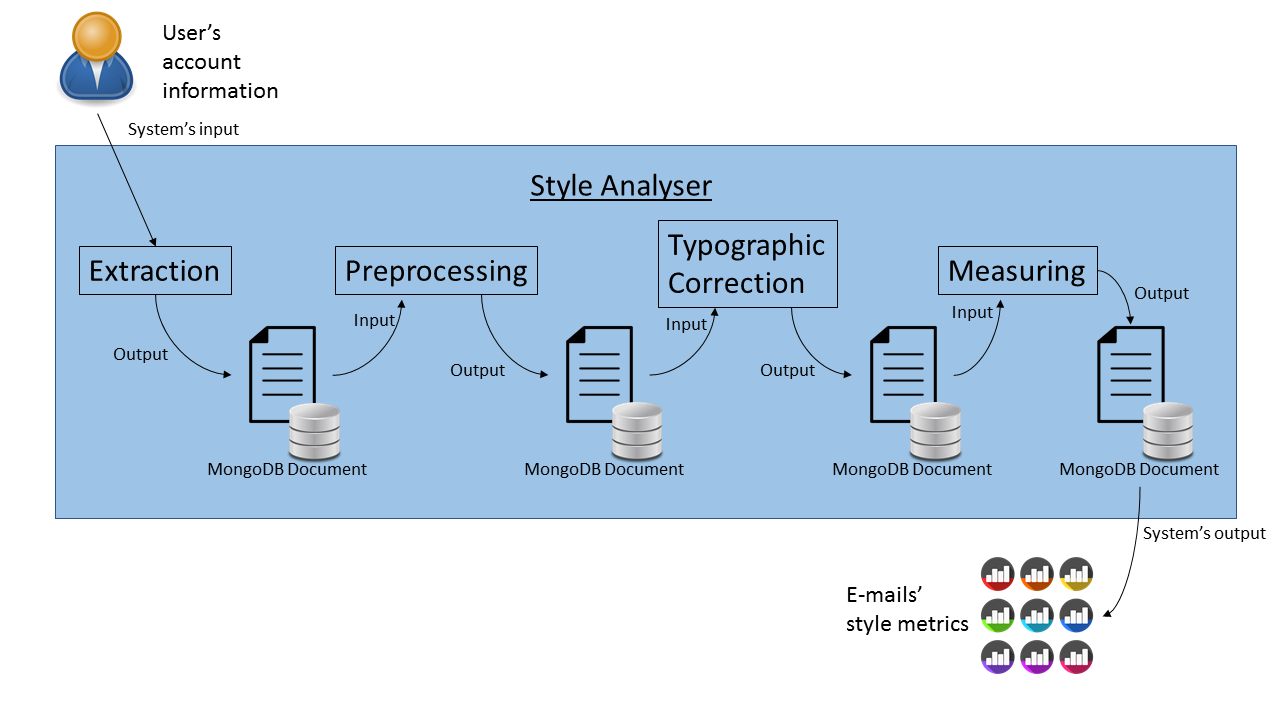
\includegraphics[width = 1.2\textwidth]{Imagenes/Bitmap/Analyser/architecture.png}}%
	\caption{Pipeline architecture of the style analyser}%
	\label{fig:arch}
\end{figure}

As it is easy to deduce, each of these phases is going to be developed as a different module. This implementation will have the advantage that each module is going to be able to work independently from the other modules, which will allow them to work in parallel. That is to say, while a message is being extracted, other e-mails could be being preprocessed, corrected or measured if they have gone through the previous phases. This optimizes the time it takes for a message to be extracted until the respective metrics are calculated (it does not have to wait for the others to move to the next phase of the pipeline). In addition, the last three (preprocessing, typographic correction and measuring) have been implemented as web services using Flask (see Section \ref{sect:flask}), which facilitates their reuse even separately in other works and projects. Let us now briefly explain what each of the defined phases consists of.

The first step, extraction phase, consists of the extraction of each one of the sent messages of the given user. In this task, we are going to take advantage of all the studied concepts about the Gmail API (see Section \ref{ssect:gmailapi}) and make use of every resource it provides us. Besides, we will try to minimize the consumed quota units in each extraction, which means we will only make the requests to the Google Servers that are strictly necessary. This first step is not just the task of extracting the resource that represents each sent message from the user's account, but also the job of transforming it to the format that the preprocessing module needs. Hence, the input of this module will be the same input as that of the complete system (information about Gmail user) and its output will be an extracted message ready for being preprocessed.

As for the second step, the preprocessing phase, consists of modifying the extracted message so that it can be interpreted by the spaCy's natural language processing model to be used. Some of the changes that a message could suffer in this phase are: the removal of the signature, the disposal of the replied messages which appears under the text, the elimination of soft break lines that quoted-printable codification (see Section \ref{sssect:quot-p}) introduce in some messages, etc. This module also addresses the need to remove characters and structures that do not correspond to those used in a plain text such as bold or italic type styles, font sizes and fonts, enumerations or bulleted lists, etc. Likewise, its output is a message with its body as a plain text.

In the implemented metrics (as we will see in section \ref{section:measmod}) we will not take into account typographical errors (such as a spelling mistake). So we will need to fix them as much as possible, and this is the typographic correction module's task. In the same way, it is possible that some tokens do not belong to our spaCy model's vocabulary. Therefore, it will be necessary to know lexical-syntactic information about the token, such as its part of speech and its lemma. These are the task of the typographic correction module.

Finally, the measuring module is in charge of calculating all the style features chosen for this work. For that purpose, it receives a message (extracted by the extracting module) with a plain text format (thanks to the preprocessing module) free from typographic error (thanks to the typographic correction module) and obtains the result of measuring all the style markers selected in the given message.

As we have explained, the input of the extracting module is information about a Gmail user and the input of the rest of the modules is a single message. However, each module is independent from each other, which means that it is necessary to have a way of assembling all this modules. For this purpose, the \textit{Analyser} class is developed (see Section \ref{sect:analyserclass}). This entity is in charge of sending to each module the required input in order to obtain its output. Moreover, it presents the system to the user, communicates the information and captures the user's information (it performs a previous filtering to check that there are no formatting errors), such as the typographic correction of the errors found. In this manner, the architecture of our style analyser system is as shown in Figure \ref{fig:umlarch} (in the following sections we will delve into each module of this system), which represents the UML (Unified Modelling Language) class diagram of it. In this figure we have avoided including both attributes and methods of each class, since with it we want to show the general structure of the system. In the sections corresponding to each of the packages and the \textit{Analyser} class, their attributes and methods will be specified and explained.

\begin{figure}[p]
	\centering%
	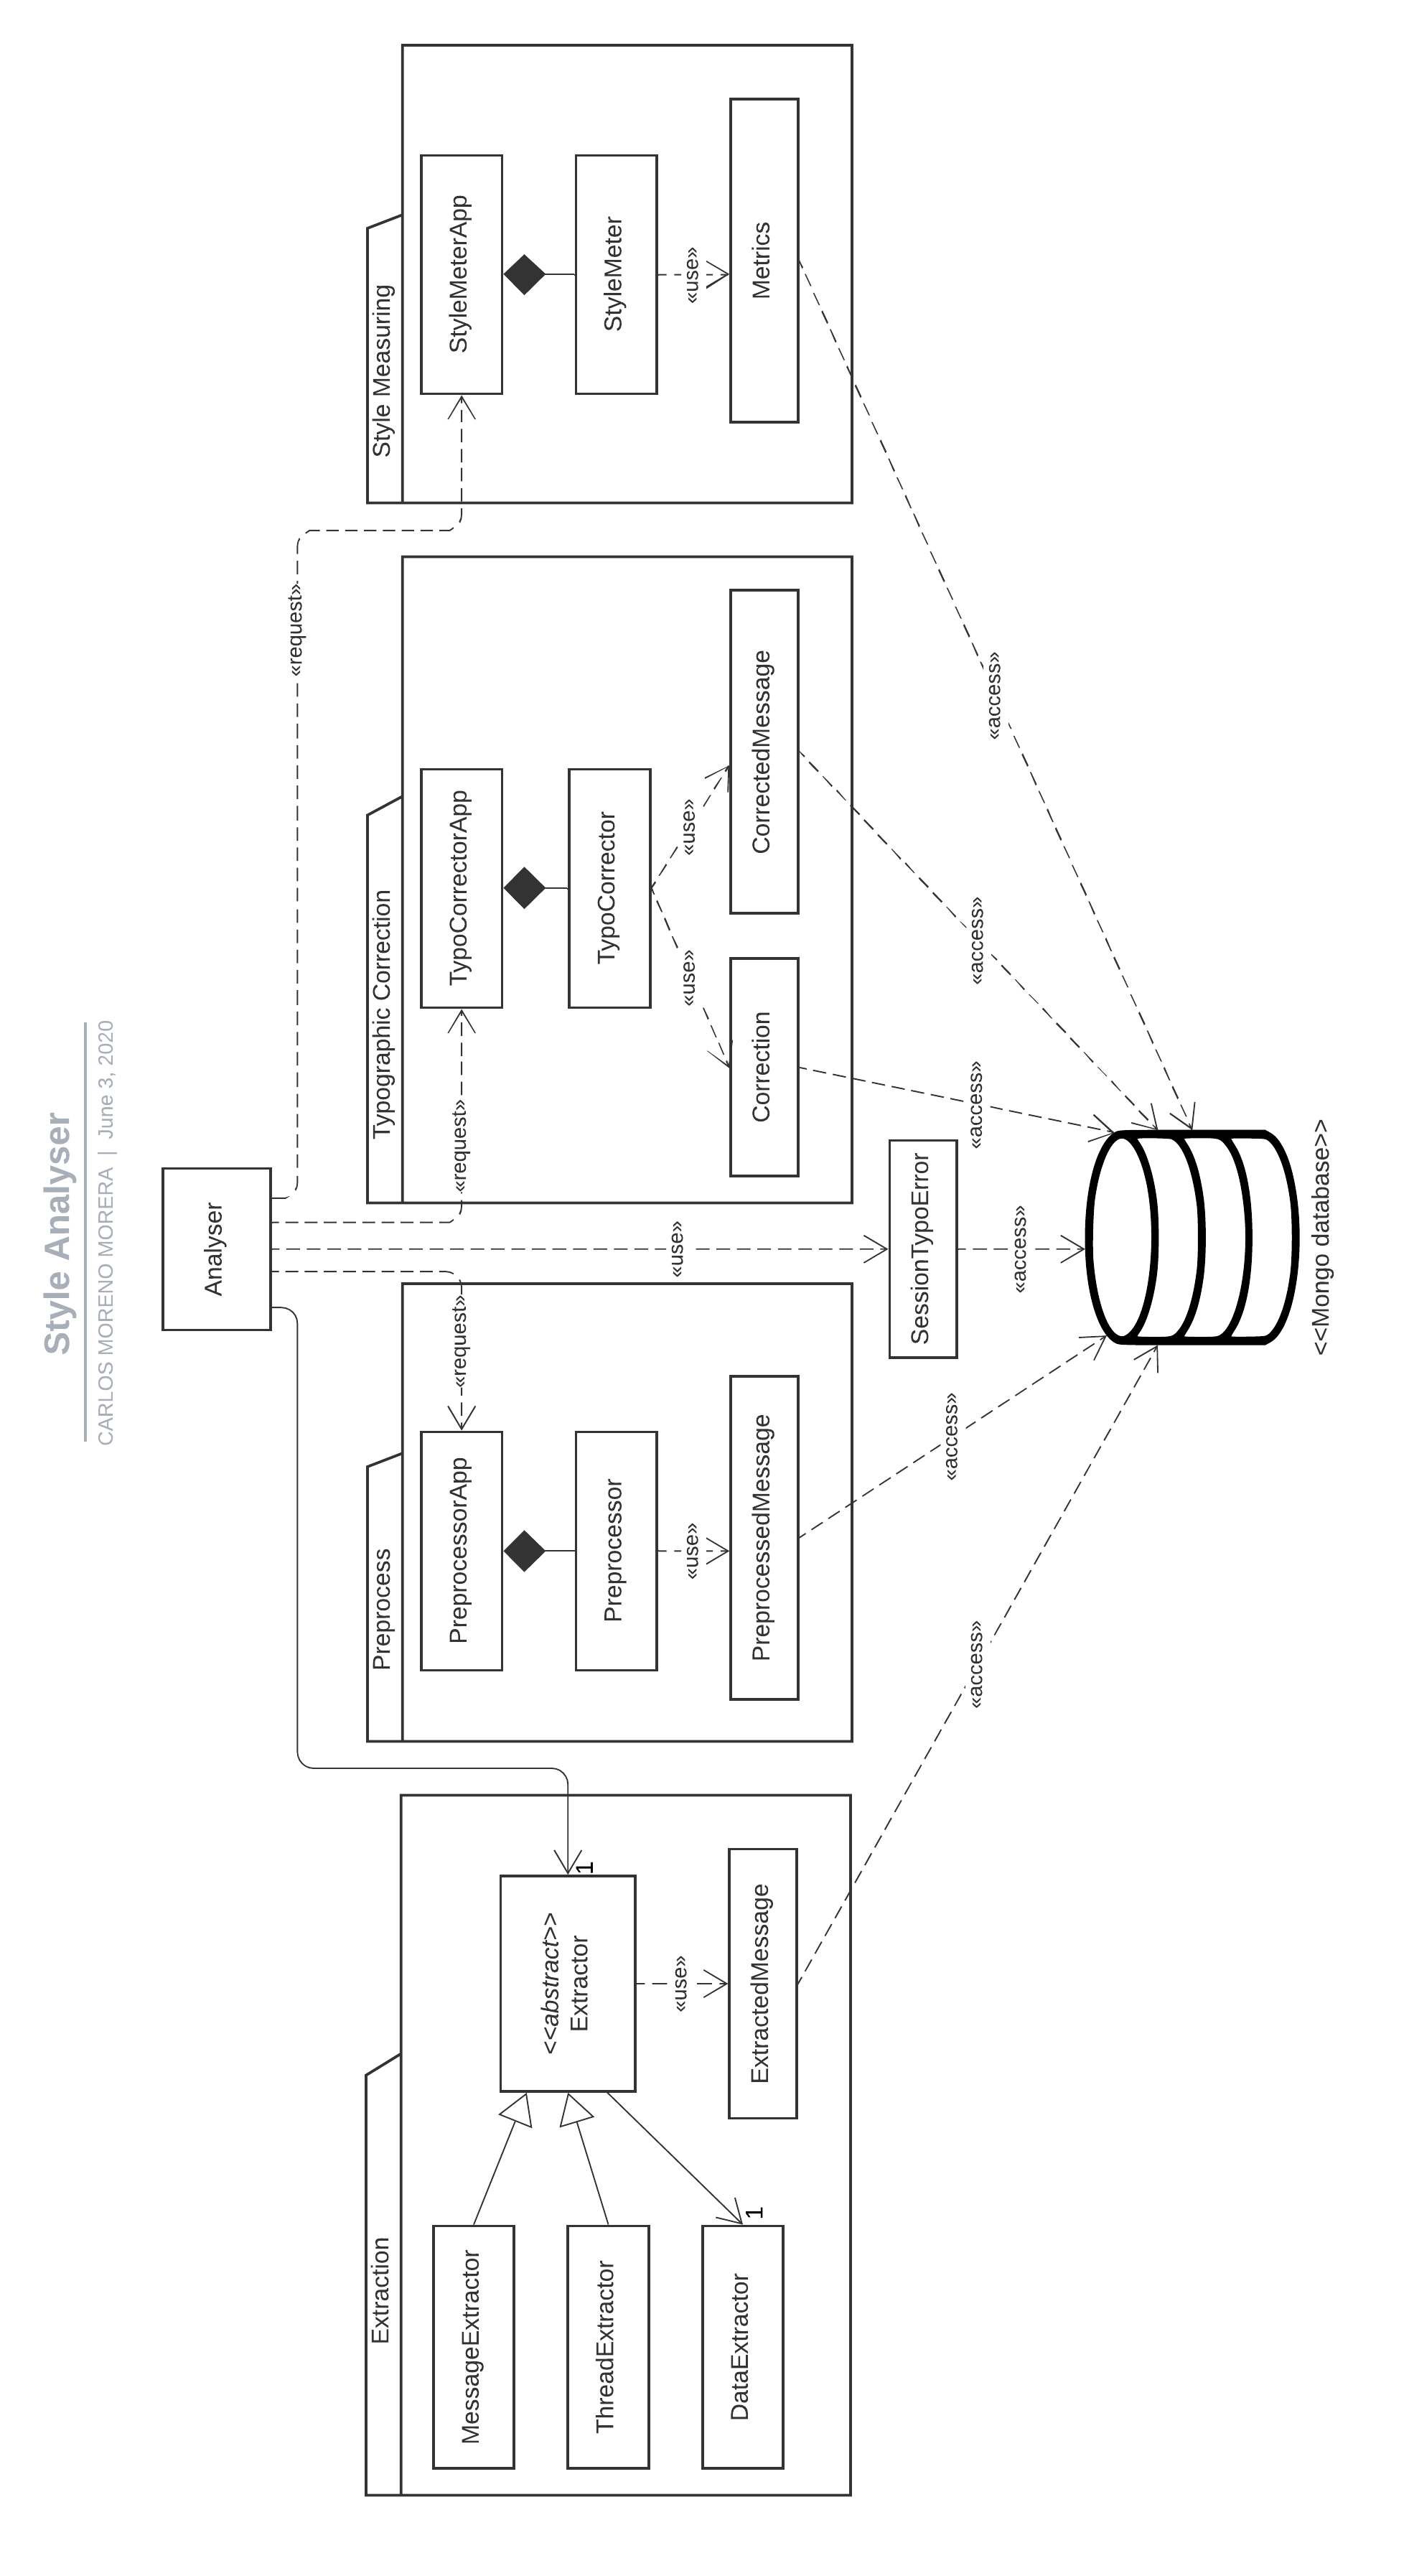
\includegraphics[height=0.85\paperheight]{Imagenes/Bitmap/Analyser/StyleAnalyserUML.png}%
	\caption{UML class diagram of the style analyser}%
	\label{fig:umlarch}
\end{figure}

As we wanted, the \textit{Analyser} manages the communication between each UML package (which represent each of the mentioned modules). Thus, this UML class will transport the output of each module to the input of the subsequent phase so as to fulfil the pipeline established in Figure \ref{fig:arch}.

If we look at the relationship shared by the \textit{Analyser} class and the \textit{Extraction} package (specifically with the \textit{Extractor} class of this module), we will notice that it is an uni-directional binary association, what it means that the objects of the second are connected with the objects of the first. Furthermore, we can observe a multiplicity index in the arrowhead (the \textit{Extraction}'s end), which means that the \textit{Analyser} will be related with an only \textit{Extractor} object (it will not be necessary to have more than one \textit{Extraction} package in order to obtain all user's sent messages).

The rest of packages are ``used'' by the \textit{Analyser}, through a POST HTTP request, because all of them are implemented as web services. It contacts with the module's app which is related with the module's main class (which is in charge of carrying out its corresponding task).

An important observation to mention is the fact that all packages interact with their corresponding classes, which act as DAO (Data Access Object), with the database used (with MongoDB technology as it is explained in Section \ref{sect:mongo}). Their interaction is based on storing their results in it. The main advantage of this implementation is that it is not required to have enough dynamic memory in order to process every message at the same time. In addition to it, as we have explained, if an error is detected in an specific phase, it is not necessary to execute the previous modules again. With this in mind, it is reasonable to think that each module's main class, of the last three phases, will make use of the corresponding class with the purpose of saving its result, obviously after finishing its execution with the given message.

Below we only have to enter in detail of each of the packages and of the \textit{Analyser}, in order to completely understand the style analyser.